
\section{Description}

The program mainly utilized the concept of arrays to return a working 10-by-10
game board. To improve user experience, visual and audio elements were added to
the program interface. This feature is the significant purpose of using a
resource called \emph{SDL} or \href{https://www.libsdl.org/}{Simple DirectMedia Layer},
to render animation, play sound, and showcase creatives.

\begin{table}[H]
    \centering
    \def\arraystretch{2.5}
    \begin{tabular}{ c c c }
        \toprule
        Instruction & Definition & Representation \\
        \midrule
        O & Pacman & 
\includegraphics[scale=0.1]{assets/pacman_sample.png} \\
        $*$ & Food & 
\includegraphics[scale=0.1]{assets/food_sample.png} \\
        X & Blocks & 
\includegraphics[scale=0.1]{assets/block_sample.png} \\
        \$ & Door & 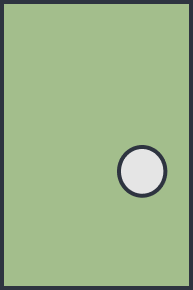
\includegraphics[scale=0.1]{assets/door_sample.png}\\
        \bottomrule
    \end{tabular}
    \caption{The visual representation of symbols in the Ghostless Pacman game}
    \label{tab:1}
\end{table}

Pacman, instead of a a plain `O', might definitely look more like Pacman. In
fact, this Pacman actually munches. Rendering its animation is a feature of the
said SDL library, which also allowed the program to display food pieces
as something more delicious than asterisks or any other punctuation, that is,
cherries. Game obstacles that look tougher than `X', and instead of a
dollar sign for the exit door, an exit door.\\

More than these, the resource is also used to render other images such as the
overall interface of the game, including the menus, prompts, and warnings.
Visual assets have been originally constructed using an online software called
\href{https://www.figma.com/}{Figma}.\\

Another use of SDL is for the incorporation of sounds and music into the game.
The audio assets used in the game are royalty-free and, if whose owner demands
copyright, are given proper credit in About the Game.\\

In terms of functions, below are some that have been integrated into the
program as the project requires:

\begin{enumerate}
    \item \codeword{fill_board_with_foods}\\
    \hspace{1em} This function will randomly fill the board with foods
    \item \codeword{fill_board_with_blocks}\\
    \hspace{1em} This function will randomly fill the board with blocks
    \item \codeword{check_if_player_won} and \codeword{check_player_status}\\
    \hspace{1em} These functions work hand-in-hand to check if the player reaches the exit sign after eating all the food pieces,
    or otherwise displays the player status of whether he or she wins or loses
\end{enumerate}

Another crucial function defined is
\codeword{count_impassable_neighbors} which helps in ensuring that any
round in the game is winnable by preventing instances such as a food piece or exit door is surrounded by blocks from all sides.\\

Other functions are described in the code itself through comments, but here are some more brief descriptions:

\begin{itemize}[label={}]
    \item \codeword{init_board} initializes the board of the game.
    \item \codeword{render_board} renders the game board including the main board, Pacman, cherries, blocks, and the exit door.
    \item \codeword{fill_board_with_exit} randomly places in the game board an exit door.
    \item \codeword{move_pacman} handles the movement of Pacman.
    \item \codeword{calculate_pacman_position} is a helper function that calculates and returns the position of Pacman.
    \item \codeword{render_state} handles the `state` of the application. It changes `state` when the player hits a wall causing a Game Over, or when the player chooses to go to the menu, etc. This function `renders` or, in other words, shows the current `state` of the application.
    \item \codeword{render_sprite} renders the various image assets needed for the game.
    \item \codeword{render_reminder} renders the image and animation of the prompts that pop up after a wrong input or choosing to exit the application.
    \item \codeword{process_keypress} handles the different keypresses made by the player during the game. This function modifies the `states` variable in accordance with the response to the various keypresses of the player.
    \item \codeword{SDL_GetTicks} is an SDL-defined function that counts the miliseconds since the function is called. This is essential for the spacing of animations involved.
    \item \codeword{SDL_Delay} is an SDL-defined function that delays execution of certain parts of the code.
    \item \codeword{Mix_FadeInMusic} is an SDL-defined function that loads the background music for the game.
\end{itemize}


The code also made use of header (.h) files to declare certain variables for
the game. Some significant concepts involved are for and while loops, structs, and
switch cases.\\

Variables used in the game are much elaborated on the lines of code at which they were used. To give an overview, here are some major ones:\\

\begin{table}[H]
    \centering
    \def\arraystretch{2}
    \begin{tabular}{ m{16em} m{25em} } 
        \toprule
        Variable & Use \\
        \midrule
        \codeword{SDL_Window *window} & A variable which manages the window of the whole application.\\
        
        \midrule
        \codeword{Board board} & 
                            An instance of the \codeword{Board} struct containing
                            variables which are related to the game itself. 
                            It contains the following members:
                            \begin{enumerate}
                                \item \codeword{array}
                                \item \codeword{number_of_blocks}
                                \item \codeword{number_of_foods}
                                \item \codeword{current_number_of_foods_picked}
                                \item \codeword{total_player_score}
                            \end{enumerate}
        \\

        \midrule
        \codeword{States states} & 
                            An instance of the struct \codeword{States} that
                            manages the state of the application 
                            It contains the following members:
                            \begin{enumerate}
                                \item \codeword{player_state}
                                \item \codeword{game_state}
                                \item \codeword{wrong_input_state}
                                \item \codeword{current_tutorial_page}
                                \item \codeword{ti}
                            \end{enumerate}
        \\
        \bottomrule
    \end{tabular}
    \caption{Major variables used in creating Ghostless Pacman}
\end{table}

% line break, kasi napuputol sa page sa haba

\begin{table}[H]
    \centering
    \def\arraystretch{2}
    \begin{tabular}{ m{20em} m{15em} } 
        Variable & Use \\
        \hline
        \codeword{player_keypress} & is a variable related to the scanning of what keys the user presses, through SDL's \codeword{SDL_Keycode}. This variable is frequently mentioned in the code, since the program mostly relies on the keypresses and inputs of the user. \\
        \codeword{wrong_input_state} & an \codeword{enum} variable that returns the current state of wrong input or keypress, specifically at which game state it occurs. States include \codeword{WRONG_INPUT_NONE}, \codeword{WRONG_INPUT_IN_MENU}, \codeword{WRONG_INPUT_IN_GAME}, \codeword{WRONG_INPUT_IN_GAME_PROMPTS}, \codeword{WRONG_INPUT_IN_ABOUT_GAME}, \codeword{WRONG_INPUT_IN_TUTORIAL}, and \codeword{WRONG_INPUT_IN_FOOD_INPUT}\\
    \end{tabular}
    \caption{(Continuation) Major variables used in creating Ghostless Pacman}
\end{table}
